\documentclass{article}
\usepackage[slovak]{babel}
\usepackage{graphicx}
\usepackage[pdf]{pstricks}
\usepackage[top=1in, bottom=1.25in, left=1.25in, right=1.25in]{geometry}

\newcommand\qadra[1][2]{%
    \psset{unit=#1pt}
    \begin{pspicture}(4,3)
        \pspolygon(0,1)(2,2.5)(4,1)(2,0.25)
    \end{pspicture}}

\begin{document}
\large
\noindent
Adam Jenča\\
Tercia A\\
SŠ Novohradská, Bratislava\\
Príklad Z9-I-2\\
\vskip 5mm \noindent
\begin{center}
	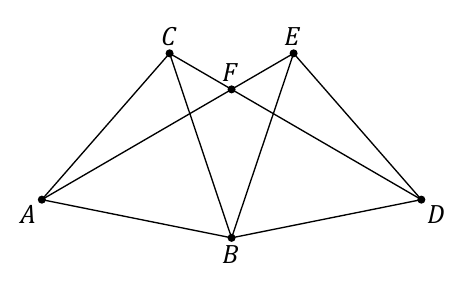
\includegraphics[scale=0.4]{xetex/imagery/wyrd}
\end{center}
\vskip 5mm
Keďže $\triangle ABC$ a $\triangle BDE$ sú zhodné rovnostranné trojuholníky, vieme, že  $\triangle ABE$ a $\triangle CBD$ sú zhodné rovnoramenné trojuholníky, a preto aj ich niektoré uhly majú rovnakú veľkosť($|\angle ABE| = |\angle CBD|$, $|\angle BAE| = |\angle AEB| = |\angle BCD| = |\angle BDC|$)
Označme si uhol $\angle ABD$ $\alpha$.\\
Vypočítajme si veľkosti uhlov $\angle ABE$ a $\angle CBD$.
$$\beta = |\angle ABE| = |\angle CBD| =  \alpha - 60$$
Teraz si vypočítajme veľkosti uhlov pri základni $\triangle ABE$ a $\triangle CBD$

$$\gamma = |\angle BAE| = |\angle AEB| = |\angle BCD| = |\angle BDC| = \frac{180-\beta}{2}$$,
pretože $\triangle ABE$ a $\triangle CBD$ sú rovnoramenné a súčet veľkostí uhlov v trojuholníku je $180^{\circ}$\\
\noindent
Odvoďme si veľkosť uhla $\angle AFD$ zo súčtu uhlov \qadra[3]$ABFD$, ktorý je pri štvoruholníkoch $360^{\circ}$.\\
$
|\angle AFD| = 360 - \alpha - 2\gamma = 360 - \alpha - 2 . \frac{180-\beta}{2} = 360 - \alpha (180 - \beta) = 360 - \alpha - [180 - (\alpha - 60)] = 360 - \alpha - 180 + \alpha - 60 = \mathbf{120^{\circ}}
$\\
\textbf{Veľkosť uhla $\mathbf{\angle AFD}$ je $ \mathbf{120^{\circ}}$}
\end{document}
